%File: formatting-instruction.tex
\documentclass[letterpaper]{article}
\usepackage{aaai}
\usepackage{times}
\usepackage{helvet}
\usepackage{courier}
\usepackage{comment}
\frenchspacing
\pdfinfo{
/Title (Formatting Instructions for Authors Using LaTeX)
/Subject (AAAI Publications)
/Author (AAAI Press)}
\setcounter{secnumdepth}{0}  

%\usepackage[letterpaper]{geometry}
 \usepackage{graphicx}
\usepackage{subfigure}
\usepackage{algorithm}
\usepackage{algpseudocode}
\usepackage{url}

\newcommand{\theHalgorithm}{\arabic{algorithm}}

\usepackage{xcolor}
\usepackage[american]{babel}
\usepackage{auto-pst-pdf}
\usepackage{microtype}
\usepackage{psfrag}
\usepackage{amsmath}
\usepackage{amssymb}
\usepackage[T1]{fontenc}
\usepackage{nicefrac}
\usepackage{booktabs}


\newcommand{\psff}[1]{\input{#1.tex}\includegraphics{#1.eps}}
\newcommand{\R}{\ensuremath{\mathbb{R}}}
\newcommand{\deq}{=}
\newcommand{\given}{\!\ensuremath{\mid}\!}
\newcommand{\cm}[1]{\ensuremath{\mathcal{#1}}}
\newcommand{\bm}[1]{\ensuremath{\mathbf{#1}}}
\newcommand{\data}{\ensuremath{\cm{D}}}
\newcommand{\inv}{\ensuremath{^{-1}}}
\newcommand{\acro}[1]{\textsc{\MakeLowercase{#1}}}

% Mike's definitions
\newcommand{\dd}[2]{\delta(#1-#2))}
\newcommand{\vect}[1]{\bm{#1}}
\newcommand{\vy}{\vect{y}}
\newcommand{\vx}{\vect{x}}
\newcommand{\vf}{\vect{f}}
\newcommand{\vs}{\vect{\sigma}}
\newcommand{\amean}[2]{\tilde{{m}}(#1 \given #2 )}
\newcommand{\acov}[2]{\tilde{{C}}(#1 \given #2 )}
\newcommand{\p}[2]{p(#1\given#2)}
\newcommand{\fPr}{p}
\newcommand{\Prob}[2]{\fPr(#1 \given #2 )}
\newcommand{\tightProb}[2]{\fPr(#1\!\given\!#2)}
\newcommand{\ps}[2]{p(#1\vert#2)}
\newcommand{\mean}[2]{{m}(#1\given#2)}
\newcommand{\cov}[2]{{C}(#1\given#2)}
\newcommand{\N}[3]{\cm{N}( #1;#2,#3 )}
\newcommand{\st}{_{\star}}
\newcommand{\tr}{\ensuremath{\mathsf{T}}}

\DeclareMathOperator{\fault}{fault}
\DeclareMathOperator{\diag}{diag}
\DeclareMathOperator{\chol}{chol}


\newcommand{\fix}{\marginpar{FIX}}
\newcommand{\new}{\marginpar{NEW}}

\newcommand{\citet}[1]{\citeauthor{#1} (\citeyear{#1})}

% \usepackage{usbib}
% \renewcommand{\citenamefont}[1]{\textsc{\MakeLowercase{#1}}}
% \renewcommand{\bibnamefont}[1]{\textsc{#1}}
% \renewcommand*{\bibname}{biblography}



\begin{document}



\title{Prediction and Fault Detection of Environmental Signals with Uncharacterised Faults}

\author{ Anonymous Author 1 \And Anonymous Author 2 \And Anonymous Author 3 \And Anonymous Author 4}

% \aistatsauthor{ Michael Osborne \And Anonymous Author 2 \And Anonymous Author 3 }
% 
% \aistatsaddress{ Department of Engineering Science\\University of Oxford\\ \url{mosb@robots.ox.ac.uk} \And Unknown Institution 2 \And Unknown Institution 3 } ]

% \icmlauthor{$^\ast$}{}
% \icmlauthor{Roman Garnett$^\dagger$}{rgarnett@andrew.cmu.edu}
% \icmlauthor{Kevin Swersky$^\ddagger$}{kevin@aquaticinformatics.com}
% \icmlauthor{Nando de Freitas$^\text{\S}$}{nando@cs.ubc.ca}
% \icmladdress{$^\ast$ \vspace{-10pt}}
% \icmladdress{$^\dagger$Department of Computer Science, Carnegie Mellon University \vspace{-10pt}}
% \icmladdress{$^\ddagger$Aquatic Informatics \vspace{-10pt}}
% \icmladdress{$^\text{\S}$Department of Computer Science, University of British Columbia}
\maketitle

\begin{abstract}
\begin{quote}
 Many signals of interest are corrupted by faults of an unknown
type. We propose an approach that uses Gaussian processes and a
general ``fault bucket'' to capture \textit{a priori} uncharacterised
faults, along with an approximate method for marginalising the
potential faultiness of all observations. This gives rise to an
efficient, flexible algorithm for the detection and automatic
correction of faults. Our method is deployed in the domain of water
monitoring and management, where it is able to solve several fault
detection, correction, and prediction problems. The method works well
despite the fact that the data is plagued with numerous difficulties,
including missing observations, multiple discontinuities, nonlinearity and many unanticipated types of fault.
\end{quote}
\end{abstract}

\section{Introduction}


Water sustainability is one of the most significant issues that
humanity faces. The quality and availability of water
directly affects the health and well-being of both human and natural
environments. Water also has a massive economic impact, affecting
industries
such as agriculture, mining, power, forestry, and more. Population and
industrial growth, along with climate change, are beginning to stress
water supplies. Between 1994 and 1999, 26\% of Canadian municipalities
reported water shortages despite the fact that Canada
contains 7\% of the world's renewable freshwater supply \cite{atlas_canada}.

One of the keys to effective water sustainability involves proper
monitoring and analysis. Water is not distributed evenly in space
and time, and being able to measure, predict, and respond to changes
in the water supply will allow organizations to allocate supplies to
where they are needed most. To this end, organizations such as Water
Survey Canada (\acro{WSC}) and the United States Geological Survey
(\acro{USGS})
have set up around 11,000 monitoring stations across North America
\cite{wagner2006guidelines}, many of them reporting telemetry data in
real-time. Analyzing this ever-increasing amount of data by hand is
difficult, costly, and time-consuming; there are many opportunities
for Machine Learning
to automate this process in order to significantly improve the
efficiency and effectiveness of current water-management systems.

In this paper, we attack the problem of
fault detection, correction, and prediction in water monitoring
signals.  Here measurements are often corrupted in non-trivial ways by
various intermittent faulty sensing and communication mechanisms,
giving rise to outliers, telemetry spikes, missing data, drift, and
multiple unanticipated exogenous disturbances (see
Figure~\ref{fig:monitoring}).  Further, signals are not well-modelled
by simple parametric approaches, such as linear or Markovian
models. Despite the enormous importance of such monitoring,
appropriate machine-learning techniques are yet to be deployed for
this purpose. In particular, there is a clear need for flexible
algorithms, able to cope with signals and faults of many different
types without placing a significant model-building burden upon
users. Such algorithms must also be able to run reliably in real-time
on incoming data.
% To accomplish this, we need to design
% techniques for detecting patterns and making predictions with
% challenging datasets, fraught with 
% %missing data, discontinuities and
% \textit{a priori} unknown types of nonlinearity and non-stationarity.
These techniques will enable us to provide operators with high-level
summaries for better decision support and, in the future, to increase
the level of automation and efficiency in water-management systems.

\begin{figure*}[t!]
\begin{center}
 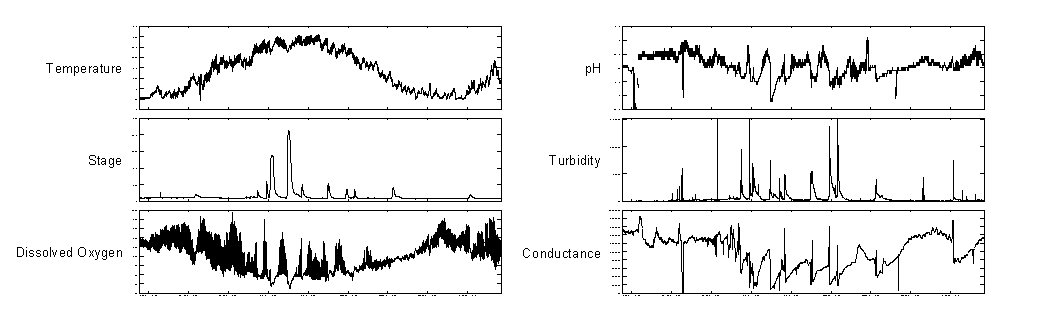
\includegraphics[width=\textwidth, height=5cm]{watermonitoring.eps}
\end{center}
\caption{16 months worth of data from six representative
signals in water quality monitoring,
which corresponds to approximately 11\,000 measurements per series.
These signals are highly nonlinear, demonstrating periodicity at
different scales,
intermittent pulses, and changes in dynamics. Not only do these
signals exhibit a wide range of dynamics,
but different signals of the same measurement type can also differ
drastically if they are taken in different regions.
}
\label{fig:monitoring}
\end{figure*}


The collection of literature on fault- (also known as novelty-, anomaly-
and one-class-) detection is vast
\cite{Eciolaza2001,deFreitas1996,Isermann2005,Ding2008,Markou2003,Chandola:2009,Khan2010,Dereszynski}.
Unfortunately, the problems solved by most of these techniques are of
very different character to our own, rendering such techniques
inapplicable. Further, after
much experimentation with those methods that are applicable (some of the results
appear in our experiments section) it became clear that off-the-shelf
techniques could not satisfy our requirements for reliable water
monitoring. This was predominately due to excessively restrictive assumptions
(e.g., that signals were linear, Markov or Gaussian), and/or a failure to
produce reasonable uncertainty
estimates. Green-tech areas, including environmental monitoring and
energy-demand prediction, are still far from full
automation; the provision of uncertainty estimates is necessary to
allow human operators to make appropriate decisions. For this reason,
we focus on developing probabilistic nonlinear models of the signal. In
addition to
providing posterior probabilities of observation faultiness, we are
able to perform effective prediction for the latent process even in
the presence of faults.

Our proposed method will rely on Gaussian processes (\acro{gp}s) due
to their flexibility and widely demonstrated effectiveness. \acro{gp}s have been used previously for
fault detection in \citet{Eciolaza2001}, but in a very different
context, unsuitable for our problem. Previous work along similar lines
has approached this problem by creating models that
specify
the anticipated potential fault types \textit{a priori}
\cite{garnettosborne}, but this is usually an unreasonable assumption
in highly variable or poorly understood environments. 
In our proposed  ``fault bucket'' approach, each point is assumed generated from either a nominal or generic faulty process; we do not require the specification of precise fault models. In
this way, our model can simultaneously identify anomalies and robustly
make predictions in the presence of sensor faults. 
% Since we cannot
% make any strong assumptions about the nature of the faults, we model
% the faulty process as a distribution with extremely high variance.
The result is an efficient method for data-stream prediction
that can manage a
wide range of faults without requiring significant
domain-specific knowledge.


% 
% 
% This approach has been effectively utilized in \cite{Dereszynski}.
% However that work uses dynamic Bayesian networks and focuses on
% integrating multiple, redundant sensors, while we focus on the
% univariate case. Our motivation for univariate modeling stems from the
% fact that water monitoring organizations, such as Water Survey Canada
% or the United States Geological Survey, often have sparse sensor
% deployments, where redundancy cannot be as easily exploited. It is
% therefore imperative that our techniques be flexible enough to apply
% to both the univariate and multivariate settings. Ideally, we would
% attempt to classify each point in the time series, and update our
% estimates as new data arrives, however for a series of length $T$ this
% has $O(2^T)$ complexity. Instead, we will introduce an effective
% approximation which as we will demonstrate,
% maintains a reasonable accuracy while keeping the computation tractable.

\section{Gaussian Processes}

Gaussian processes provide a simple, flexible framework for performing
Bayesian inference about functions \cite{gpml}.  A Gaussian process
is a distribution on the functions $f\colon \cm{X} \to \R$ (on an
arbitrary domain $\cm{X}$) with the property that the distribution of
the function values at a finite subset of points $F \subseteq \cm{X}$
are multivariate Gaussian distributed. A Gaussian process is completely defined by its first two moments: a
mean function $\mu\colon \cm{X} \to \R$ and a symmetric positive
semidefinite covariance function $K\colon \cm{X} \times \cm{X} \to
\R$.  The mean function describes the overall trend of the function
and is typically set to a constant for convenience.  The covariance
function describes how function values are correlated as a function of
their locations in the domain, thereby encapsulating information about
the overall shape and behavior of the signal.  Many covariance
functions are available to model a wide variety of anticipated
signals.

Suppose we have chosen a Gaussian process prior distribution on the
function $f\colon \cm{X} \to \R$, and a set of input points $\bm{x}$,
the prior distribution on $\bm{f} \deq f(\bm{x})$ is
\begin{equation*}
 p(\bm{f} \given \bm{x}, \theta)
 =
 \cm{N}
 \bigl(
   \bm{f};
   \mu(\bm{x}; \theta),
   K(\bm{x}, \bm{x}; \theta)
 \bigr),
\end{equation*}
where $K(\bm{x}, \bm{x}; \theta)$ is the Gram matrix of the points
$\bm{x}$, and $\theta$ is a vector containing any parameters required
of $\mu$ and $K$, which form hyperparameters of the model.

Exact measurements of the latent function are typically not available.
% however,
%  we may combine the Gaussian process distribution on the
% latent function with an observation model that takes into account
% potential noise in our measurements.  
Let $y(x)$ represent the
value of an observation of the signal at $x$ and $f(x)$
represent the value of the unknown true latent signal at that point.
When the observation mechanism is not expected to experience faults,
the usual noise model used is
\begin{equation}\label{iidnoise}
 p(y \given f, x, (\sigma^n)^2)
 \deq
 \cm{N}(y; f, (\sigma^n)^2),
\end{equation}
which represents additive i.i.d.\space Gaussian observation noise with
variance $(\sigma^n)^2$. Note that this model is inappropriate when
sensors can experience faults, which corrupt the relationship
between $y$ and $f$.

With the observation model above, given a set of observations
$
 \data
 \deq
 \bigl\lbrace
   \bigl( x, y(x) \bigr)
 \bigr\rbrace
 \deq
 ( \bm{x}, \bm{y} )
$,
the posterior distribution (itself given by a Gaussian Process) of $f\st \deq f(x\st)$ given these data is
\begin{equation}\label{eq:GP_posterior}
 p(f\st \given \vy, \theta)
 =
 \cm{N}
 \bigl(
   f\st;
   \mean{f\st}{\vy,\theta},
   \cov{f\st}{\vy,\theta}
 \bigr),
\end{equation}
where the posterior mean and covariance are
\begin{align*}
 &
 \mean{f\st}{\vy,\theta}
 \deq
 \mu(x\st; \theta)
 +
 K(x\st, \bm{x}; \theta)
V \inv
 \bigl(
   \bm{y} - \mu(\bm{x}; \theta)
 \bigr)
 \\  
 &
 \cov{f\st}{\vy,\theta}
 \deq
 K(x\st, x\st; \theta)
 -
 K(x\st, \bm{x}; \theta)
 V\inv
 K(\bm{x}, x\st; \theta),
\end{align*}
for $ V \deq 
 K(\bm{x}, \bm{x}; \theta) + (\sigma^n)^2 \bm{I}
 $.

We now make some definitions for the sake of readability. Henceforth,
we assume that our observations $\vy$ have already been scaled by the
subtraction of the prior mean $\mu(\bm{x}; \theta)$. We will also make
use of the covariance matrix shorthand $K_{m,n} \deq
K(\vx_m,\vx_n)$. Finally, for now, we'll drop the explicit dependence
of our probabilities on the hyperparameters $\theta$ (it will be
implicitly assumed that all quantities are conditioned on knowledge of
them) and will return to them later. Similarly, we drop the dependence of our probabilities on the values of inputs $x$, which we assume are always known.

\section{Fault Bucket}\label{bucket}

We propose an algorithm that is designed to deal with faults of many different, unspecified types. We use a sequential scheme, applicable for ordered data such as time series, partitioning the data available at any point into old and new halves.  We then approximately marginalise the faultiness of old observations, storing and then updating our results for future use. This gives rise to an efficient and fast algorithm. In order to effect our scheme, we make four key approximations:
\begin{enumerate}
 \item \label{app:fb} {\bf Fault bucket:} Faulty observations are assumed to be generated from a Gaussian noise distribution with a very wide variance.
\item \label{app:single_gaussian} {\bf Single-Gaussian marginal:} A mixture of Gaussians, weighted by the posterior probabilities of faultiness of old data, is approximated as a single moment-matched Gaussian.
\item \label{app:independence} {\bf Old/new noise independence:} We assume that noise contributions are independent, and that the contributions for new data are independent of old observations.
\item \label{app:affine} {\bf Affine precision:} The precision matrix over both old and new halves is assumed to be affine in the precision matrix over the old half.
\end{enumerate}
Approximations \ref{app:fb} and \ref{app:single_gaussian} represent the state-of-the-art \cite{Dereszynski}. However, using them alone will not give an algorithm that can scale to the real-time problems we consider. Our novel approximations \ref{app:independence}-\ref{app:affine} permit very fast, fault-tolerant inference. We will detail and justify these approximations further below.

Our single, catch-all, ``fault bucket'' is expressed by approximation \ref{app:fb}. It is built upon the expectation that points that are more likely to have been generated by noise with wide variance than under the normal
predictive model of the \acro{gp} can reasonably be assumed to
be corrupted in some way, assuming we have a good understanding of the
latent process. It is hoped that a very broad class of faults can be
captured in this way. 
To formalise this idea, we choose an observation noise distribution to
replace \eqref{iidnoise} that models the noise as independent
but not identically distributed with separate variances for the
non-fault and fault cases:
\begin{align}
\begin{split}\label{eq:observation_likelihood}
  p(y \given f, x, \neg\fault, (\sigma^n)^2)
 &
 \deq
 \cm{N}(y; f, (\sigma^n)^2)
 \\
 p(y \given f, x, \fault, (\sigma^f)^2)
 &
 \deq
 \cm{N}(y; f, (\sigma^f)^2),
\end{split}
\end{align}
where $\fault \in \lbrace 0, 1 \rbrace$ is a binary indicator of
whether the observation $y(x)$ was faulty and $\sigma^f > \sigma^n$ is
the standard deviation around the mean of faulty measurements.  The
values of both $\sigma^n$ and $\sigma^f$ form hyperparameters of our
model and are hence included in $\theta$.

Of course, {\it a priori}, we do not know whether an
observation will be faulty.  Unfortunately, managing our uncertainty
about the faultiness of all observations is a
challenging task. With $N$ observations, there are $2^N$
possible assignments of faultiness; it is infeasible to consider them all. Our solution is founded upon approximation \ref{app:single_gaussian}. We approximately marginalise the faultiness of old observations, representing the mixture of different Gaussian predictions (each given by a different combination of faultiness) as a single Gaussian. This natural approach is similar to that taken in the related field of switching Kalman filters \cite{murphy1998switching}. We prefer this approximate marginalisation over
faultiness to heuristics that would designate
observations as either faulty or not---we acknowledge our
uncertainty about faultiness. 

More formally, define $\vs$ to be the (unknown) vector of
all noise variances at observations $\vy$. Because we have to sum over all possible values for these
vectors, we will index the possible values of
$\vs$ by $i$, each given by a different combination of
faultiness over $\data$ (e.g. $\vs_t^0=\vs^n$ for $\neg\fault$ and $\vs_t^1=\vs^f$ for $\fault$).
Given all data $\data$, we need to marginalise over predictions indexed by $i$, as per
\begin{align}
& \p{f\st}{\vy} \nonumber\\
& = \sum_{i} \Prob{\vs^i}{\vy} \p{f\st}{\vy, \vs^{i}} \nonumber\\
& =\sum_{i} \Prob{\vs^i}{\vy} \cm{N}\bigl(f\st; \mean{f\st}{\vy, \vs^{i}}, \cov{f\st}{\vy, \vs^{i}}\bigr),\label{eq:Gaussian_marginal}
\end{align}
the weighted sum of Gaussian predictions made using the different
possible values for $\vs$. By moment-matching, we collapse the weighted sum of all these predictions to a single Gaussian prediction. 

In order to build a sequential algorithm, imagine that we have partitioned our observations
$\data_{a,b}$ into a set of old observations
$\data_a\deq(\vx_a,\vy_a)$ and a set of new observations $\data_b
\deq (\vx_b,\vy_b)$. We will index the possible values of
$\vs_{a}$ by $i$ and the values of $\vs_{b}$ similarly by
$j$. We now define the covariance matrices over our data
%\begin{align*}
 $V_a^i  \deq K_{a,a} + \diag \vs_{a}^i$,
 $V_b^j  \deq K_{b,b} + \diag \vs_{b}^j$ and
 $V_{a,b}^{i,j} \deq K_{\{a,b\},\{a,b\}} + \diag \{\vs_{a}^i,\vs_{b}^j\}$,
%\end{align*}
where $\diag \vs$ is the diagonal matrix with diagonal $\vs$. From \eqref{eq:GP_posterior}, we know that our predictions have relatively simple dependence upon the inverse of $V$, the precision. To approximate \eqref{eq:Gaussian_marginal} as a single Gaussian, a simple calculation reveals that we require\footnote{Actually, with some rearrangement, we can avoid explicitly computing (unstable) matrix
inverses and instead work with Cholesky factors to solve the required linear equations.} the expected values of $V^{-1}$ and $V^{-1}y y^\tr V^{-1}$, expectations with respect to $\Prob{\vs^i}{\vy}$.  
We'll refer to the set of those two expected values (which are matrices) as the \emph{marginal set}, which, given $\data_a$, we denote as $M_a$. Our approach relies upon storing $M_a$, and then performing simple updates in order to arrive at $M_{a,b}$, the marginal set given $\data_{a,b}$. Hence our approximate marginalisation from previous time steps can be efficiently used to determine an approximate marginalisation for the current time step. 

% It is our hope that our predictions
% for $f\st$ are not so sensitive to the noise in our observations that
% all our Gaussian predictions, one become dramatically different. In any
% case, the quality of this approximation will improve over time---if
% $f\st$ is far removed from our old data $\data_a$, then our
% predictions really will not be very sensitive to $\sigma_a$. 

This approach firstly relies upon approximation \ref{app:independence}; we assume that faults will not persist longer than $|\data_b|$. To be precise, we assume
\begin{equation} \label{eq:approx}
p(\vs^{i,j}_{a,b},\vy_{a,b})  \simeq p(\vs^i_{a})\,\Prob{\vy_a}{\vs^i_{a}}\,
%P
p(\vs^j_{b})\,\p{\vy_b}{\vs^{i,j}_{a,b},\vy_{a}}
\end{equation}
This simplifies the expectations required to evaluate $M_{a,b}$. A further simplification is afforded by approximation \ref{app:affine}, in which we assume that
$({V}^{i,j}_{a,b})^{-1}$ is effectively affine in $(V^i_a)^{-1}$. This
is true if given $\data_b$, it is impossible to accurately predict
$\data_a$. This might be the case if $\data_a$ represents a lot of
information relative to $\data_b$ (if, for example, $\data_a$ is our
entire history of observations where $\data_b$ is simply the most
recent observation), or if $\data_b$ and $\data_a$ are simply not
very well correlated. Together, approximations \ref{app:independence} and \ref{app:affine} allow us the efficient updates to $M$ required to build an online algorithm.

The further laborious mathematical details of the derivation of our algorithm are omitted for clarity. An outline of our approach is depicted in algorithm \ref{alg:fault_bucket}.

\begin{comment}


To initialise our algorithm, imagine that $a$ identifies a small set
of data, such that we can readily compute the likelihood of our hyperparameters
\begin{equation}
 \hspace{-0.0cm}p(\vy_a)\!=\!\sum_i  \ps{\vy_a}{\vs^i_a}\fPr(\vs^i_a)
\!=\! \sum_i \N{\vy_a}{0}{V_a^i}\fPr(\vs_a^i) \label{eq:likelihood_a}
\end{equation}
and hence the hyperparameter posterior, $\ps{\vs_a}{\vy_{a}}$.
% \begin{equation*}
% \ps{\vs_a}{\vy_{a}} 
% = \frac{\ps{\vy_a}{\vs_a}\fPr(\vs_a)}{p(\vy_a)} 
% = \frac{\N{\vy_a}{0}{V_a} \fPr(\vs_a)}{p(\vy_a)}\label{eq:psa}.
% \end{equation*}
This distribution specifies the probability of our observations
$\data_a$ being faulty; for a single observation $\data_a$,
$
p\bigl(\fault(\data_a) \given \vy_{a}\bigr) = \Prob{\sigma_a = \sigma^f}{\vy_{a}}
$.
If we were to perform predictions for some $f\st$ using $\data_a$
alone, we would need to evaluate
\begin{align*}
& \p{f\st}{\vy_{a}} \\
& = \sum_{i} \Prob{\vs^i_{a}}{\vy_a} \p{f\st}{\vy_a, \vs^{i}_{a}} \\
& =\sum_{i} \Prob{\vs^i_{a}}{\vy_a} \cm{N}\bigl(f\st; \mean{f\st}{\vy_a, \vs^{i}_{a}}, \cov{f\st}{\vy_a, \vs^{i}_{a}}\bigr),
\end{align*}
the weighted sum of Gaussian predictions made using the different
possible values for $\vs_{a}$.  We now use approximation \ref{app:single_gaussian}. It is our hope that our predictions
for $f\st$ are not so sensitive to the noise in our observations that
all the Gaussians in this sum become dramatically different. In any
case, the quality of this approximation will improve over time---if
$f\st$ is far removed from our old data $\data_a$, then our
predictions really will not be very sensitive to $\sigma_a$. So, we take
\begin{align*}
& \p{f\st}{\vy_{a}} \simeq
\cm{N}\bigl(f\st; K_{\star,a} \tilde{V}_a^{-1} \vy_a, 
\\ & \hspace{1cm}
K_{\star,\star} - K_{\star,a}(\tilde{V}_a^{-1}-\tilde{W}_a^{-1})K_{a,\star} 
 - (K_{\star,a} \tilde{V}_a^{-1}\vy_a)^2\bigr),%\label{eq:pya}
\end{align*}
% where we have
% \begin{align}
% \amean{f\st}{\vy_{a}} \deq {}& K_{\star,a} \tilde{V}_a^{-1} \vy_a,\label{eq:ameana}\\
% \acov{f\st}{\vy_{a}}
% \deq {}& K_{\star,\star} - K_{\star,a}(\tilde{V}_a^{-1}-\tilde{W}_a^{-1})K_{a,\star} 
%  - \amean{f\st}{\vy_{a,b}}^2 ,\label{eq:acova}
% \end{align}
where\footnote{
Note that for $\tilde{W}_a$, explicitly computing (unstable) matrix
inverses can be avoided by solving the appropriate linear equations
using Cholesky factors.  For $\tilde{V}_a$, we can rewrite
$(A^{-1}+B^{-1})^{-1} = A (A+B)^{-1} B$. If $i\in\{0,1\}$ (as it would
be if $a$ identified a single observation which could be either faulty
or not),
\begin{align} \label{eq:inverse_trick}
\tilde{V}_a & = V^0_a\bigl(
\Prob{\vs^1_{a}}{\vy_a} V^0_a 
+ 
\Prob{\vs^0_{a}}{\vy_a} V^1_a
\bigr)^{-1}V^1_a.
\end{align}
If $i$ takes more than two values, we can simply iterate using the
same technique. We can then use the Cholesky factor of $\tilde{V}_a$ to compute our required equations.}
\begin{align}
 \tilde{V}_a^{-1}  & \deq \sum_i \Prob{\vs^i_{a}}{\vy_a} (V_a^i)^{-1},\nonumber\\
 \tilde{W}_a^{-1} & \deq \sum_i \Prob{\vs^i_{a}}{\vy_a} (V_a^i)^{-1}\vy_a \vy_a^\tr (V_a^i)^{-1}.\label{eq:Wa}
\end{align}
% Having computed
% $\tilde{V}_a$, we can then calculate
% \begin{align} %labelled only for alg statement
%  \tilde{R}_a & \deq \chol \tilde{V}_a \\%\label{eq:Ra}, \\ 
%  \tilde{T}_a & \deq \chol (\tilde{R}_a)^{-1} \vy_a %\label{eq:Ta},
% \end{align}
% and use them, with \eqref{eq:Wa}, to determine
% \eqref{eq:ameana} and \eqref{eq:acova}.
With these calculations performed, imagine receiving
further data $\data_b$. To progress, we make approximation \ref{app:independence}; we assume that faults will not persist longer than $|\data_b|$. To be precise, we assume
\begin{equation} \label{eq:approx}
p(\vs^{i,j}_{a,b},\vy_{a,b})  \simeq p(\vy_a)\,\Prob{\vs^i_{a}}{\vy_a}\,
%P
p(\vs^j_{b})\,\p{\vy_b}{\vs^{i,j}_{a,b},\vy_{a}}
\end{equation}
Our predictions are now
\begin{multline}
\p{f\st}{\vy_{a,b}} %= \sum_{i} \sum_{j} \p{f\st}{\vy_{a,b}, \vs^{i,j}_{a,b}} \Prob{\vs^{i,j}_{a,b}}{\vy_{a,b}}.
\simeq 
% {}& \sum_{j} \Prob{\vs^j_{b}}{\vy_{a,b}}\sum_{i} \Prob{\vs^i_{a}}{\vy_a} \p{f\st}{\vy_{a,b}, \vs^{i,j}_{a,b}}\nonumber\\
% = {}&
\sum_{j} \Prob{\vs^j_{b}}{\vy_{a,b}}\sum_{i} \Prob{\vs^i_{a}}{\vy_a} \\
 \cm{N}\bigl(f\st; \mean{f\st}{\vy_{a,b}, \vs^{i,j}_{a,b}}, \cov{f\st}{\vy_{a,b}, \vs^{i,j}_{a,b}}\bigr).\label{eq:sum_o_Gaussians}
\end{multline}
Before trying to manage these sums, we will determine $p(\vs_b \given \vy_{a,b})$. As before, this distribution gives us the probability
of the observations $\data_b$ being faulty. For example, if we have
only a single observation $\data_b$, $
p\bigl(\fault(\data_b) \given \vy_{a,b}\bigr) = \Prob{\sigma_b =
  \sigma^f}{\vy_{a,b}} $. We define
\begin{align*}%labelled only for alg statement
\amean{\vy_b}{\vy_a} \deq {} &
K_{b,a} \tilde{V}_a^{-1} \vy_a %\label{eq;ameanba}
\\
\acov{\vy_b}{\vy_{a},\vs_b}
\deq {} & V_b - K_{b,a}(\tilde{V}_a^{-1}-\tilde{W}_a^{-1})K_{a,b} \nonumber\\
 & \hspace{3cm} - \amean{\vy_b}{\vy_{a,b}}^2, %\label{eq;acovba}
\end{align*}
where both $\tilde{V}_a$ (or its Cholesky factor) and
$\tilde{W}_a^{-1}$ were computed previously. By using
approximations \ref{app:single_gaussian} and \ref{app:independence},
\begin{align*}
\Prob{\vs_b}{\vy_{a,b}} & = \frac{\sum_i \p{\vy_b}{\vy_a,\vs^i_{a,b}}p(\vy_a,\vs^i_{a,b})}{p(\vy_{a,b})} 
\nonumber\\
% \simeq \frac{\sum_i \p{\vy_b}{\vy_a,\vs^i_{a,b}}\fPr(\vs_a^i\mid{\vy_a})\fPr(\vs_{b})}{\ps{\vy_{b}}{\vy_a}}
& \simeq \frac{\cm{N}\bigl(\vy_b; \amean{\vy_b}{\vy_a}, \acov{\vy_b}{\vy_a, \sigma_b}\bigr) \fPr(\vs_b)}{\p{\vy_{b}}{\vy_a}},%\label{eq:psb}
\end{align*}
where we have
\begin{align*}
p(\vy_{b} \given \vy_a)
& = \sum_i \sum_j \p{\vy_b}{\vy_a,\vs^i_{a,b}}\Prob{\vs^{i,j}_{a,b}}{\vy_a}
\nonumber\\
% \simeq \sum_i \sum_j \p{\vy_b}{\vy_a,\vs^i_{a,b}}\Prob{\vs_a^i}{\vy_a}\fPr(\vs_{b}^j)
&  \simeq \sum_j \cm{N}\bigl(\vy_b; \amean{\vy_b}{\vy_a}, \acov{\vy_b}{\vy_a, \vs_b^j}\bigr) \fPr(\vs_b^j).%\label{eq:likelihood_b}
\end{align*}
Note that the product of $p(\vy_{b} \given \vy_a)$ and $p(\vy_a)$ (previously computed in
\eqref{eq:likelihood_a}) gives the likelihood of our hyperparameters. Now, returning to \eqref{eq:sum_o_Gaussians}, we will once again
use approximation \ref{app:single_gaussian}. We aim to reuse our previously evaluated sums over
$i$ to resolve future sums over $i$. As we gain more data, the
faultiness of old data becomes less important. We arrive at
\begin{align*}
&\p{f\st}{\vy_{a,b}} \simeq \cm{N}\bigl(
f\st;\ 
K_{\star,\{a,b\}} \tilde{V}_{a,b}^{-1} \vy_{a,b},
\\ & \hspace{0.1cm}
K_{\star,\star} - K_{\star,a}(\tilde{V}_{a,b}^{-1}-\tilde{W}_{a,b}^{-1})K_{a,\star} - (K_{\star,\{a,b\}} \tilde{V}_{a,b}^{-1} \vy_{a,b})^2
\bigr)\,,%\label{eq:pyab}
\end{align*}
where we have
\begin{align*}
% \amean{f\st}{\vy_{a,b}} \deq {}&  %\label{eq:ameanab}
% \\
% \acov{f\st}{\vy_{a}}
% \deq {} &  \\%\label{eq:acovab}
% % \end{align*}
% % \vspace{-0.8cm}
% % \begin{align*}
\tilde{V}^{-1}_{a,b} \deq {} &
\sum_{j} \Prob{\vs^j_{b}}{\vy_{a,b}}\sum_i \Prob{\vs^i_{a}}{\vy_{a}} (V_{a,b}^{i,j})^{-1} \\
\tilde{W}^{-1}_{a,b} \deq {} &
\sum_{j} \Prob{\vs^j_{b}}{\vy_{a,b}}\sum_i \Prob{\vs^i_{a}}{\vy_{a}} 
\\
& \hspace{3cm}
(V_{a,b}^{i,j})^{-1}  
 \vy_{a,b}^{\phantom{\tr}} \vy_{a,b}^\tr (V_{a,b}^{i,j})^{-1}.
\end{align*}
Now, using the inversion by partitioning formula \cite[Section 2.7]
{NumericalRecipes},
\begin{align*}
&
({V}^{i,j}_{a,b})^{-1} =
\\
& \hspace{-0.2cm}
\begin{bmatrix}
 S^{i,j}_a &\hspace{-0.1cm} -S^{i,j}_a K_{a,b} (V^j_b)^{-1} \\
 - (V^j_b)^{-1} K_{b,a} S^{i,j}_a &\hspace{-0.1cm} (V^j_b)^{-1}\!+\!(V^j_b)^{-1} K_{b,a} S^{i,j}_a K_{a,b} (V^j_b)^{-1} 
\end{bmatrix}
\end{align*}
where
$
S^{i,j}_a \deq (V^i_a -K_{a,b} (V^j_b)^{-1}K_{b,a})^{-1}\,.
$ Note that $({V}^{i,j}_{a,b})^{-1}$ is affine in $S^{i,j}_a$, so that when $V_a \gg K_{a,b} V_b^{-1} K_{b,a}$,
% \begin{equation}\label{eq:V_a_big}
%  V_a \gg K_{a,b} V_b^{-1} K_{b,a}\,,
% \end{equation}
$({V}^{i,j}_{a,b})^{-1}$ is effectively affine in $(V^i_a)^{-1}$. This
is true if given $\data_b$, it is impossible to accurately predict
$\data_a$. This might be the case if $\data_a$ represents a lot of
information relative to $\data_b$ (if, for example, $\data_a$ is our
entire history of observations where $\data_b$ is simply the most
recent observation), or if $\data_b$ and $\data_a$ are simply not
particularly well correlated. On this basis, we make approximation \ref{app:affine}. Additionally noting that $\sum_i \Prob{\vs^i_{a}}{\vy_{a}} = 1$, we have
\footnote{
$\tilde{V}^{-1}_{b|a}$ can be computed using the same trick as in \eqref{eq:inverse_trick} if
$b$ identifies a single observation and $j\in\{0,1\}$. The Cholesky factor of $\tilde{V}_{a,b}$ required to solve the linear equations for our predictions can be efficiently determined 
\cite{OsborneAnon}
%\cite[Appendix B]{osbornebayesian} 
using the previously evaluated Cholesky factor of $\tilde{V}_{a}$.
}
\begin{align*}
\tilde{V}^{-1}_{a,b} &\simeq \sum_j \Prob{\vs^j_{b}}{\vy_{a,b}} \begin{bmatrix}
 \tilde{V}_a & K_{a,b}
\\
 K_{b,a} & V^j_b
\end{bmatrix}^{-1},
\nonumber\\
\tilde{V}_{a,b} & \simeq
\begin{bmatrix}
 \tilde{V}_a & K_{a,b}\\
 K_{b,a} & \tilde{V}_{b|a} + K_{b,a} \tilde{V}_a^{-1} K_{a,b}
\end{bmatrix}\\
%  Defining the affine map $f\colon (V^i_a)^{-1}
% \mapsto ({V}^{i,j}_{a,b})^{-1}$, then, noticing $\sum_i \Prob{\vs^i_{a}}{\vy_{a}} = 1$,
% $$
% \sum_i \Prob{\vs^i_{a}}{\vy_{a}} f\bigl((V^i_a)^{-1} \bigr) \simeq f\Bigl(\sum_i \Prob{\vs^i_{a}}{\vy_{a}}(V^i_a)^{-1} \Bigr).
% $$
% 
% where
% \begin{equation*}
 \tilde{V}^{-1}_{b|a} & \deq \sum_j \Prob{\vs^j_{b}}{\vy_{a,b}} (V^j_b -K_{b,a} \tilde{V}_a^{-1}K_{a,b})^{-1}\,.
\end{align*}
 Note that the
lower right hand element of $\tilde{V}_{a,b}$ defines the noise
variance to be associated with observations $\data_b$. In effect, we represent
each observation as having a known variance lying between
$(\sigma^n)^2$ and $(\sigma^f)^2$. The more likely an observation's
faultiness, the closer its assigned variance will be to the (large)
fault variance and the less relevant it will become for inference
about the latent process. This approximate observation is then used
for future predictions; we need never consider the full sum over all
observations. 

We now turn to $\tilde{W}_{a,b}^{-1}$. Unfortunately, even if
$V_a \gg K_{a,b} V_b^{-1} K_{b,a}$, $\tilde{W}_{a,b}^{-1}$ is quadratic in
$(V^i_a)^{-1}$. We will nonetheless again make approximation \ref{app:affine} and assume that $\tilde{W}_{a,b}^{-1}$
is affine in $(V^i_a)^{-1}$. The quality of our approximation for
$\tilde{W}_{a,b}^{-1}$ is much less critical than for
$\tilde{V}^{-1}_{a,b}$, because the former only influences the
variance of our predictions for the current predictant; any flaws in
that approximation will not be propagated forward. Further, of course,
if one probability dominates, 
%\begin{equation*}
$
\Prob{\vs^i_{a}}{\vy_{a}}\gg
\Prob{\vs^{i'}_{a}}{\vy_{a}}, \forall i' \neq i,
$
%\end{equation*} 
then the approximation is valid. With this,
\begin{align*}
\tilde{W}^{-1}_{a,b} \simeq
& \sum_{j} \Prob{\vs^j_{b}}{\vy_{a,b}} 
\\
& \hspace{0.5cm}
\begin{bmatrix}
 \tilde{V}_a & K_{a,b}
\\
 K_{b,a} & V^j_b
\end{bmatrix}^{-1}\vy_{a,b}^{\phantom{\tr}}\, \vy_{a,b}^\tr \begin{bmatrix}
 \tilde{V}_a & K_{a,b}
\\
 K_{b,a} & V^j_b
\end{bmatrix}^{-1}\,.%\label{eq:Wab}
\end{align*}
If we now receive further data $\data_c$, our existing data is simply treated as old data ($a \leftarrow \{a,b\}$, $b \leftarrow c$), and another iteration of our algorithm performed.
% and we can solve for
% $K_{\star,(a,b)}\tilde{W}^{-1}_{a,b}K_{(a,b),\star}$ by efficiently
% updating using the previously computed quantity $\tilde{T}_{a}$.
\end{comment}

\begin{algorithm}[tb]
   \caption{Fault Bucket}
\label{alg:fault_bucket}
\begin{algorithmic}[1]
\Statex{{\bfseries Input:} data $(\vx,\vy)$, lookahead $\delta$, fault prior $\pi$.}
\Statex{{\bfseries Output:} 
posterior probabilities of faultiness $\p{\sigma^1_t}{\vy_{1:t}}$, likelihoods $p(\vy_{1:t})$, predictions $\p{f_{t+\delta}}{\vy_{1:t}}$.}
\State $x_a \leftarrow x_1,\, y_a \leftarrow y_1,
\,x\st \leftarrow x_{1+\delta}$
\State {\bfseries return:} $p(y_a) \leftarrow$\\
\hfill\acro{marginal-gp-predictions}$(y_a, x_a, \pi)$
\For{$i = 0,1$}
\State {\bfseries return:} $\Prob{\vs^i_a}{y_{a}} \leftarrow$ 
\acro{fault-posterior$\bigl(p(y_a), \pi\bigr)$}
\EndFor
 \State $M_a \leftarrow$ 
\acro{marginal-set}$\bigl(y_a, x_a,  \{\Prob{\vs^i_a}{y_{a}}\}\bigr)$
\State {\bfseries return:} $\p{f\st}{y_{a}} \leftarrow$
\acro{marginal-gp-predictions}\\
\hfill$\bigl(x\st, y_a,  x_a, \{\Prob{\vs^i_a}{y_{a}}\}, M_a\bigr)$
\For{$t = 2,\ldots$}
\State $x_b \leftarrow x_t, y_b \leftarrow y_t, x\st \leftarrow x_{t+\delta}$
\State $\p{y_b}{\vy_a} \leftarrow$ 
\acro{marginal-gp-predictions}\\
\hfill$\bigl(y_b, x_b, y_a, x_a, \pi, M_a\bigr)$
\State {\bfseries return:} $p(\vy_{a,b}) \leftarrow p(\vy_a)\p{\vy_b}{\vy_a}$
\For{$j = 0,1$}
\State {\bfseries return:} $\Prob{\vs^j_b}{\vy_{a,b}} \leftarrow$
\acro{fault-posterior}\\\hfill$\bigl(p(\vy_{a,b}), \pi\bigr)$
\EndFor
\State $M_{a,b} \leftarrow$
\acro{update-marginal-set}\\
\hfill$\bigl(\vy_{a,b},\vx_{a,b},\{\Prob{\vs^j_b}{\vy_{a,b}}\},M_a\bigr)$
\State {\bfseries return:} $\p{f\st}{\vy_{a,b}}\leftarrow$ 
\acro{marginal-gp-}\\
\hfill\acro{predictions}$\bigl(x\st,\vy_{a,b}, \vx_{a,b},  \{\Prob{\vs^j_b}{\vy_{a,b}}\},M_{a,b}\bigr)$
\State $p(\vy_{a}) \leftarrow p(\vy_{a,b})$
\State $\vx_a \leftarrow \vx_{a,b},\, y_a \leftarrow \vy_{a,b}$
\State $M_a \leftarrow M_{a,b}$
\EndFor 
\end{algorithmic}
\end{algorithm}


\subsection{Discussion}

We return to the management of our hyperparameters
$\theta$. Unfortunately, analytically marginalising $\theta$ is
impossible. Most of the hyperparameters of our model can be set by
optimising their likelihood on a large training set, giving a
likelihood close to a delta function. This is not true of the
hyperparameters $\sigma^n$ and $\sigma^f$, due to exactly the same
problematic sums discussed earlier. Instead, we marginalise these
hyperparameters online using Bayesian Monte Carlo \cite{BZMonteCarlo,OsborneIPSN}, %\cite[Chapter 7]{osbornebayesian},
taking a fixed set of samples in their values
and using the hyperparameter likelihoods $p(\vy_{a,b})$ to construct
weights over them. Essentially, we proceed as described above
independently in parallel for each sample, and combine the predictions
from each in a final weighted mixture for prediction. Note that we can
use a similar procedure \cite{garnettosborne} to determine the full
posterior distributions of $\sigma^n$ and $\sigma^f$, if desired.  It
would be desirable to use non-fixed samples, but, unfortunately, this
would require reconstructing our full covariance matrix from
scratch each time a sample is moved.

Our proposal can be extended in several ways. First, we may wish
to sum over more than one fault variance, useful if
observations are prone to faultiness in more than one mode.  If, instead of summing over a small number of known variances, we
wished to marginalise with respect to a density over noise variance,
we can simply replace the sums over $i$ and $j$ with appropriate
integrals. Obviously this will only be analytically possible if the
posteriors for $\sigma_a^i$ take appropriate, simple forms.  In such a way our algorithm might tackle the general problem of
heteroscedasticity.


Our proposed algorithm steps through our data one at a time, so that
$\data_b$ always contains only a single observation. 
With approximation \ref{app:independence}, this means that our algorithm is not expecting faults to last more than a single observation. The results that follow, however, will show that we can nonetheless manage sustained faults. 
It would also
be possible to step in larger chunks, evaluating larger
sums. Although more computationally demanding, this might be expected
to improve results. It would also allow us to consider non-diagonal
noise contributions.

We have so far not specified our prior for faultiness (as expressed by
$p(\sigma_a)$ and $p(\sigma_b)$). Within this paper, we consider
exclusively a time-independent probability $\pi$ of faultiness, but our framework does not necessarily require this to be so. 

In some contexts it might be useful to perform inference about the
fault contribution, rather than the signal of interest.  To do so, we merely switch the roles of the fault and non-fault
contributions. Note that, using our full posteriors for faultiness, we
can also trivially use Bayesian decision theory to make hard decisions
as required.
% To make a prediction about a potential faulty signal
% at $x$, we follow exactly the same procedure as above, substituting
% $(\sigma^n)^2$ for $(\sigma^f)^2$.

% \begin{figure*}
%   \centering
%   \small
%   \psff{bias}
%   \psff{kf_bias}
%   \vspace*{2\baselineskip}
%   \psff{dynamics}
%   \psff{kf_dynamics}
%   \caption{Mean and $\pm3\sigma$ standard-deviation bounds for the
%     predictions of (first and third) the fault-bucket algorithm and
%     (second and fourth) the Kalman filter algorithm on (top two) the
%     synthetic bias dataset and (bottom two), the synthetic anomaly
%     dataset.  Detected faults are marked in black crosses, and the
%     unobserved true values are marked in grey circles.}
%   \label{compare}
% \end{figure*}


\begin{figure*}[t]
  \centering
  \small
  \begin{tabular}{cc}
    \hspace*{2em} \textsc{xgp} -- pH & 
    \hspace*{2em} \textsc{xgp} -- painting
    %\vspace*{1ex}
    \\
    \psff{ph_exhaust} & \psff{painting_exhaust} \\
    %\\
    \hspace*{2em} \textsc{fb} -- pH & 
    \hspace*{2em} \textsc{fb} -- painting
    %\vspace*{1ex}
    \\
    \psff{ph} & \psff{painting} \\
    %\\
    \hspace*{2em} \textsc{fb} --  $p(\text{fault}(t) \given \cm{D})$ & 
    \hspace*{2em} \textsc{fb} --  $p(\text{fault}(t) \given \cm{D})$ 
    %\vspace*{1ex}
    \\
    \hspace*{-0.7em} \psff{ph_fault} & \psff{painting_fault} \\
  \end{tabular}
  \caption{Mean and $\pm3\sigma$ standard-deviation bounds for the
    predictions of the exhaustive (\textsc{xgp}) and fault-bucket
    (\textsc{fb}) algorithms on the pH and painting datasets.  For the
    fault-bucket algorithm, the posterior faultiness of each
    observation is also shown underneath the predictions.  Note that
    each column shares the same $x$-axis.}
  \label{justfb}
\end{figure*}


% Finally, some applications might required a hard decision about
% whether a particular observation was faulty.  This would be necessary,
% for example, if a system had correctional or responsive actions that
% it could take when such an event occurred.  Fortunately, we can
% address this problem using simple Bayesian decision theory.

\section{Results}
We test the effectiveness of the fault bucket algorithm on several time-series
that are indicative of problems found in environmental
monitoring. In particular, we test on water-level readings; such data
are often characterised by complex dynamics and will therefore provide
a good indicator of our algorithm's performance on real-world
tasks. We aim to improve upon the simple, human-supervised approaches
to fault detection used in this field
\cite{wagner2006guidelines}. For a quantitative assessment, we used two semi-synthetic datasets
where a typical fault has been injected into clean sensor data. We
then analyzed qualitative performance on two real data sets with actual
faults. All measurements (other than for pH) are given in meters, with samples spaced in
increments of approximately 30 minutes. %The datasets are described below.

%% We return to the water-level signal with the painting artifacts
%% plotted in Figure \ref{hgriver}.  To test the method described above,
%% we performed 10-step lookahead online prediction on the river-level
%% function using a zero-mean Gaussian process prior distribution and the
%% fault-bucket observation model.  The covariance function was chosen to
%% be a Mat\'{e}rn covariance with parameter $\nu = \nicefrac{5}{2}$
%% \cite{gpml}.  The hyperparameters of the non-fault model (the
%% characteristic input and output scales and the noise variance
%% $(\sigma^n)^2$) were learned offline via maximum-likelihood--II
%% estimation on a disjoint segment of uncorrupted data.  The fault
%% variance $(\sigma^f)^2$ was set to $0.2$ and the fault prior $\alpha$
%% was chosen to be $10\%$.

%% Figure \ref{faultpredictions} shows the results.  The predictions
%% follow the true signal much better than the model that generated the
%% results in Figure \ref{normalpredictions}.  Additionally, the model
%% detected the faulty observations with reasonable accuracy, despite the
%% very small amount of prior knowledge about faults that the
%% fault-bucket model incorporates beyond ``faulty observations are
%% unpredictable.''

%\subsubsection{Synthetic bias fault}
Our first synthetic example, a bias fault, concerns a simple sensor
error where measurements are temporarily adjusted by a constant
offset, but otherwise remain accurate. This could happen if the sensor
undergoes physical trauma which results in a loss of calibration.
%\subsubsection{Synthetic anomaly}
The next dataset contains a synthetic anomaly where the water level
rises quickly, but smoothly, before returning back to normal. This
would be indicative of a genuine environmental event such as a flash
flood. Both synthetic datasets represented sustained faults, of length 335 and 161 observations respectively.
%\subsubsection{pH}
Our first real dataset deals with pH measurements from the United States Geological Survey, a common indicator of water quality. In this series, a clear sensor fault can be seen
in which the observations undergo a sudden, sustained decrease in value.
%\subsubsection{Painting}
The next (real) dataset contains a fault type called ``painting,'' 
an error that occurs when ice builds on a sensor, obscuring some of the
readings. It is characterised by frequent sensor spikes interlaced
with the original, and still accurate, signal.
% %\subsubsection{``Fishkiller''}
% Our final (real) dataset, which we dub ``fishkiller'', comes from a sensor
% near a dam on a river in British Columbia, Canada. It contains an
% otherwise normal water level-reading that is occasionally interrupted
% by a short period of rapid oscillation. This occurs when dam operators
% open and close the floodgates too quickly, leading to rapid water level drops followed by salmon becoming stranded and suffocating. Detecting these events is critical
% to proper regulation of dams. 

%\subsection{Implementation}

We implemented the algorithm described in Section \ref{bucket} in
\textsc{matlab} to address the task of 1-step-lookahead time-series
prediction.  A sliding window of size 100 was used to predict the
value of the next observation.  Each dataset was recentered so that a
zero prior mean function was appropriate, and the functions were all
modeled using a Mat\'{e}rn covariance with parameter $\nu =
\nicefrac{5}{2}$ \cite{gpml}.  The hyperparameters for this
covariance, including the normal observation noise
$\sigma^n$, were learned using training data similar to but disjoint from the test datasets.  The unknown fault noise $\sigma^f$
was marginalised using Bayesian Monte Carlo, with a parsimonious 7 samples used.  The prior probability of an observation being faulty, $\pi$, was
set to a constant value of 1\% throughout.


\begin{table*}[t]
  \centering
  \caption{Quantitative comparison of different algorithms on the
    synthetic datasets.  For each dataset, we show the mean squared error
    (\textsc{mse}), the log likelihood of the true data ($\log p(\bm{y}
    \given \bm{x})$), and the true-positive and false-positive rates
    of detection for faulty points (\textsc{tpr} and \textsc{fpr}),
    respectively, with all methods permitted a `burn-in' period of 50 points. The best value for each set of results is highlighted in
    bold.}\vspace{0.3cm}
  \label{tbl:results}
  \begin{tabular}{ccccccccc}
    \toprule
& \multicolumn{4}{c}{Bias dataset} & \multicolumn{4}{c}{``Flash-flood'' dataset}\\
    \cmidrule(l){2-5} \cmidrule(l){6-9}
    Method & \scshape{mse} & $\log p(\bm{y}\given\bm{x})$ & \scshape{tpr} & \scshape{fpr} 
& \scshape{mse} & $\log p(\bm{y}\given\bm{x})$ & \scshape{tpr} & \scshape{fpr} \\
\midrule
    \scshape{fb} & \textbf{0.024} & 334 & \textbf{0.997} & 0.031 & 0.069 & $-5.77\times 10^3$ & \textbf{0.829} & {0.016} \\
    \scshape{xgp} & 0.037 & \textbf{439} & 0.982 & {0.022} & \textbf{0.042} & $\mathbf{-1.52 \times 10^3}$ & 0.805 & 0.012 \\
\scshape{epgp} & 0.879 & $-5.06 \times 10^3$ & 0.009 & 0.025 
	       & 2.179 & $-2.14 \times 10^4$ & 0.000 & \textbf{0.000} \\ 
    \scshape{tgp} & 0.033 & 278 & \textbf{0.997} & 0.031 & 0.075 & $-8.29\times 10^3$ & \textbf{0.829} & 0.083 \\
   \scshape{stgp} & 0.189 & $-604$ & 0.994 & 0.255 &
		  0.249 & $-1.01\times 10^5$ & 0.787 & 0.140\\
%    \scshape{argp} & 2.340 & $-1.93 \times 10^9$ & 0.6 & 0.4 & 1.097 & $-7.52\times 10^8$ & 0.178 & 0.822 \\
    \scshape{mlh} & 0.940 & $-5.43\times 10^7$ & 0.065 & 0.031 & 2.369 & $-2.27\times 10^7$ & 0.045 & 0.262 \\
%    \scshape{kf} & 0.894 & $-7.11 \times 10^5$ & 0.053 & 0.073 & 0.360 & $-3.54 \times 10^4$ & 0.835 & 0.046 \\
   \scshape{ekf} & 0.060 & $-1.26 \times 10^4$ & 0.551 & 0.258 & 0.613 & $-1.81\times 10^4$ & 0.169 & 0.768 \\
   \scshape{skf} & 0.101 & $-1.04 \times 10^4$ & \textbf{0.997} & \textbf{0.000} & 0.162 & $-3.83\times 10^4$ & 0.805 & 0.004 \\
    \bottomrule
  \end{tabular}
\end{table*}

We tested against a number of different methods in order to establish the efficacy of the fault bucket algorithm. All \acro{gp}-based approaches used the same hyperparameters employed by our algorithm. The training set used to learn those hyperparameters was also supplied to other methods for their respective model learning phases. Several methods identify a new observation $y$ as a fault if
\begin{equation}\label{eq:thresh}
 \bigl\lvert y-\mean{y}{\vy} \bigr\rvert > 3\sigma^T\,,
\end{equation}
where $\mean{y}{\vy}$ is the method's \emph{a priori} prediction for $y$, and $\sigma^T$ is the noise standard deviation on the faultless training set. Of course, methods using \eqref{eq:thresh} or similar can not provide the posterior probability of a point's faultiness, as our algorithm can. Methods tested include:

%\begin{description}
%\item[ XGP] 
{\bf XGP:}
A  \acro{gp} in which we exhaustively search over the faultiness of the last 10 points, and approximate the noise variance of all previous points in the window as having the value $(\sigma^f)^2 \p{\fault}{\vy} + (\sigma^n)^2 \p{\neg\fault}{\vy}$, fixed at the time the point was observed (when data $\data$ was available). Clearly, this method is very much more computationally expensive than the fault bucket algorithm (roughly $2^9$ times more), but offers a useful way to quantify the influence of approximations \ref{app:single_gaussian}--\ref{app:affine}.

{\bf EPGP:}
A \acro{gp} with our observation likelihood \eqref{eq:observation_likelihood} and the posterior determined by expectation propagation \cite{minka2001expectation}. Note that expectation propagation will not readily give us a posterior probability of faultiness; for the purposes of explicitly identifying faults, we use \eqref{eq:thresh}.

% \item[ TGP] 
{\bf TGP:}
A \acro{gp} in which a point was flagged as a fault using \eqref{eq:thresh}; if faulty, a point was treated as having noise variance $(\sigma^f)^2$.

{\bf STGP:}
A \acro{gp} with student-t likelihood with four degrees of freedom (found to optimise performance); the posterior was determined using a Laplace approximation as per \citet{vanhatalo2009gaussian}. To identify faults, \eqref{eq:thresh} was used.

%  \item[ ARGP] An auto-regressive Gaussian process (over the last 10 points), with a point identified as faulty using \eqref{eq:thresh}. If faulty, the value for the observation $y$ is taken as $\mean{y}{\vy}$ for future predictions.

%\item[MLH] 
{\bf MLH:} 
The most likely heteroscedastic  \acro{gp} \cite{kersting2007most}. 
%  \item[KF] A Kalman filter to perform one-step-lookahead predictions in an online fashion. Any datum identified as a fault by the threshold \eqref{eq:thresh} is simply ignored and discarded.

{\bf EKF:}
%\item[EKF] 
An autoregressive neural net trained with the extended Kalman filter to capture nonstationarity. Again, \eqref{eq:thresh} was used to identify and discard faulty data.
%\end{description}

{\bf SKF:}
%\item[EKF] 
A switching Kalman filter \cite{murphy1998switching}, which switched between the non-faulty and faulty observation models in \eqref{eq:observation_likelihood}. The model was trained by solving the Yule-Walker equations; the best model order found was three. 

Note that for \acro{epgp}, \acro{stgp} and \acro{mlh}, we perform retrospective prediction (so that all data is available to make predictions about even the first predictant), as these methods are usually used. Clearly this allows these approaches an unfair predictive advantage relative to sequential methods. Note also that the multiple passes over the data effected by approximation schemes such as expectation propagation cannot be readily applied to the sequential problem without requiring a great deal of expensive computation. For $N$ observations, the computational cost of expectation propagation is $\mathcal{O}(N^3)$, with a large constant of proportionality, rendering it impractical for real-time problems. With efficient Cholesky factor updates, our scaling is $\mathcal{O}(N^2)$. For this reason, we did not consider even more demanding, non-sequential, expectation propagation approaches such as the twinned \acro{gp} \cite{naish2008robust}. Note also that these approaches do not provide posterior probabilities of faultiness, as our method is able to. 

% TGP: GP in which a pt was flagged as a fault if |pt - p4Mean| > thresh
% XnGP: GP in which we exhaustively search over the faultiness of the last n pts, and approximate the noise variance of all previous points as having the value sigma_f p(fault|D) + sigma_n p(not fault|D), fixed at the time the point was observed (when data D was available). XnGP is more computationally expensive than FB (roughly 2^n times more)
% ARGP: Auto-regressive GP (over the last 10 pts), with a pt flagged as a fault if |pt - pMean| > thresh. If faulty, pMean is used as the value for that pt in future predictions
% EKF: Autoregressive neural net trained with the extended Kalman filter to capture nonstationarity
% MLH: Most likely heteroscedastic GP of Kersting. Retrospectively looks at all data at once instead of sequentially (which would be very slow)


%\subsection{Results}
Figures \ref{justfb} show the performance of the
fault-bucket algorithm and the exhaustive alternative on the two real datasets. The fault-bucket algorithm did an excellent
job of identifying faults when they occur, and made excellent
predictions, even for the sustained fault in the pH dataset. 

Table \ref{tbl:results} displays quantitative measures of performance
for the various algorithms on the synthetic
datasets.  
% The performance is remarkably better under mean-squared
% predictive error as well as the likelihood of the actual data.  
In addition to superior predictive performance, our
detection rates for the faulty points are generally excellent. Note that approaches that provided comparable fault-detection rates, like the \acro{tgp} and \acro{skf}, perform significantly poorer prediction.
The results reveal that approximations \ref{app:single_gaussian}--\ref{app:affine} do not result in significant loss of performance relative to exhaustive search. Our na\"{i}ve approach to faults may, of course, suffer relative to better-informed models, but its probabilistic estimates of faultiness provide a human operator with an indication as to whether more sophisticated analysis is necessary.



\section{Conclusion}
We have proposed a novel algorithm, the ``fault bucket,'' for managing
time-series data corrupted by faults of type unknown ahead of time. Our chief
contribution is a sequential algorithm for marginalising the
faultiness of observations in a \acro{gp} framework, allowing for
fast, effective prediction in the presence of unknown faults. Unlike most robust regression approaches (such as those using student-t likelihoods), we can also compute the posterior probability of faultiness. This capacity is crucial to its utility for the domain, serving as a means of alarming a human operator to the possible need for corrective action. 

As to future work, addressing multivariate signals is of great interest. Unfortunately, this extension is not trivial and would itself require additional approximations. 

%\small
\bibliographystyle{aaai}
\bibliography{fault_bucket_icml_2011}


\end{document}


